\chapter{運動の三法則}

{\small 注: この章を理解するには, 数学リメディアル教材で
「微分」「ベクトル」「微分方程式」を理解していることが必要である。}\\

これから我々は物体の運動に関する物理学を学ぶ。「物体の運動」とは, 
物体の位置や向きや形状が時刻とともに変化する様子である。
とはいうものの, 当面は「位置」だけに着目し, 「向き」や「形状」
については難しすぎるので後回しにする。そのために我々は
まず物体を質点としてモデル化し, 質点の運動を考える。

\begin{faq}{\small\textgt{てことは, 物体が変形したり回転したり
する様子はわからない, ってことですか? そんなのしょぼ過ぎません?}
... 大丈夫。質点の運動をきっちり理論化できたら, それを使って
変形や回転なども理論化できます(そのうち学びます)。物事には順序
というものがあるのです。}\end{faq}

というわけで, 我々の当面の目標は, 質点の位置を時刻の関数として
表すことだ。それには, ベクトル, 微分, 積分という3つの数学を駆使する。
まずその準備をしよう。\\


\section{ベクトルとスカラー}

中学校理科で学んだように, 速度や力は, 「向き」と「大きさ」を持つ。
このように, 向きと大きさを持つ量のことを「ベクトル」と呼ぶ(定義)。
それに対して, 大きさだけを持ち向きを持たない(ただしプラスとマイナスは
あってもよい)ような量を「スカラー」と呼ぶ(定義)。例えば力はベクトルだが, 
「力の大きさ」はスカラーである。

ベクトルを記号で表すときは, 高校では$\vec{F}$とか$\vec{v}$の
ように, 「アルファベットに上付き矢印」を使っていたが, 大学では, 
${\bf F}$とか${\bf v}$のように, 「アルファベットの太字」
を使う(慣習)。それに対して, スカラーは, 上矢印もつけず, 太字でもない, 
普通の細字のアルファベットで表す(慣習)。

ベクトルとスカラーをきっちり区別しないと, 数学的な取り扱い
で大きなミスをする可能性がある。そこでこのように, 
\begin{itembox}{慣習}
ベクトルの記号は太字\\
スカラーの記号は細字
\end{itembox}
で書き分けるのである。

物理学では, 質点の位置もベクトルとして表す。すなわち, まず空間の
どこかに「原点」を設定し, この原点から見た「向き」と「距離」で, 位置を
表す。そう考えるといろいろ便利だからである。

そのようなベクトルを「位置ベクトル」という。位置ベクトルは, 慣習的
に${\bf r}$で表すことが多い。

ベクトルは, 3次元空間の中の座標軸の方向, 
すなわち$x$方向, $y$方向, $z$方向のそれぞれの大きさ
(の組み合わせ)として表すこともできる。そういうのを「成分」
という。例えば, ${\bf F}$を力のベクトルとすると, これは
\begin{eqnarray}
{\bf F}=(F_x, F_y, F_z)\label{eq:FFxFyFz}
\end{eqnarray}
のように, 3つの成分$F_x$, $F_y$, $F_z$の組み合わせ
で表すことができる。

ベクトルの成分はスカラーである(向きがあらかじめ決められているので, 
大きさしか意味を持たない)。従って成分は細字で書かねば
ならない。つまり, \eref{eq:FFxFyFz}の左辺の${\bf F}$は太字であり, 
右辺の$F_x$, $F_y$, $F_z$は細字である。\eref{eq:FFxFyFz}を, 
\begin{eqnarray*}
&&F=(F_x, F_y, F_z)\quad\quad\text{と書いてはダメだし, }\\
&&{\bf F}=({\bf F}_x, {\bf F}_y, {\bf F}_z)\quad\quad\text{と書いてもダメ}
\end{eqnarray*}
である。\mv

\begin{faq}{\small\textgt{力はベクトルなので, 太字で書かなきゃ
ダメなんですよね。でも, 前の章では, $F=-kx$みたいに, 細字で
書いてましたが...?} ... それはバネに関するフックの法則ですね。
バネは普通, 1方向にしか伸び縮みしません。その方向に$x$軸をとり, 
それに垂直な方向に$y$軸, $z$軸をとれば, 力${\bf F}$は
\begin{eqnarray}
{\bf F}=(F_x, 0, 0)
\end{eqnarray}
と書けますね($x$軸方向以外の成分はいつもゼロ)。てことは, $y$方向
や$z$方向のことを気にする必要が無いから, 改めて$F_x$を$F$と書いて, 
\begin{eqnarray}
{\bf F}=(F, 0, 0)
\end{eqnarray}
と書いても差し支えありません。で, この$x$成分を取り出したのが, 
$F=-kx$の左辺の$F$なのです。すなわち, 常にひとつの方向(ひとつの直線の上)
に限定された現象を考える場合は, その方向での成分だけをいきなり
取り出して, 細字で書くのが普通です。これは慣習的なことですが, 
学生がよく混乱するので, 大きく書いておきましょう:
\begin{itembox}{慣習}
直線上に限定した議論や問題では, ベクトルであっても細字記号を使う。
\end{itembox}
}\end{faq}


\section{位置・速度・加速度}

\underline{位置を時刻で微分したものを速度という(定義)}。また, 
\underline{速度を時刻で微分したものを加速度という(定義)}。これらを数式で表現してみよう:

まず, 時刻を$t$とし, 質点の位置を
\begin{eqnarray}
{\bf r}(t)=(x(t), y(t), z(t))
\end{eqnarray}
とする。以後, $(t)$は, 「これは$t$の関数だ」というしるしであり, \textgt{時には省略されることもある}。

また, 質点の速度を
\begin{eqnarray}
{\bf v}(t)=(v_x(t), v_y(t), v_z(t))
\end{eqnarray}
とし, 質点の加速度を
\begin{eqnarray}
{\bf a}(t)=(a_x(t), a_y(t), a_z(t))
\end{eqnarray}
とする。そして速度と加速度を, それぞれ
\begin{eqnarray}
&&{\bf v}(t)=\frac{d}{dt}{\bf r}(t)\label{eq:v_drdt}\\
&&{\bf a}(t)=\frac{d}{dt}{\bf v}(t)=\frac{d^2}{dt^2}{\bf r}(t)\label{eq:a_dvdt}
\end{eqnarray}
と定義する。

\begin{faq}{\small\textgt{この$\frac{d}{dt}$って何ですか?}
 ... 変数$t$で微分する, という意味の記号です。数学リメディアル教材参照。}\end{faq}

\eref{eq:v_drdt}を各成分にわけて書き改めると, 以下のようになる:
\begin{eqnarray}
&&v_x(t)=\frac{d}{dt}x(t)\label{eq:def_vx_dxdt}\\
&&v_y(t)=\frac{d}{dt}y(t)\label{eq:def_vy_dydt}\\
&&v_z(t)=\frac{d}{dt}z(t)\label{eq:def_vz_dzdt}
\end{eqnarray}
また, \eref{eq:a_dvdt}を各成分にわけて書き改めると, 以下のようになる:
\begin{eqnarray}
&&a_x(t)=\frac{d}{dt}v_x(t)=\frac{d^2}{dt^2}x(t)\label{eq:def_ax_dvdt}\\
&&a_y(t)=\frac{d}{dt}v_y(t)=\frac{d^2}{dt^2}y(t)\\
&&a_z(t)=\frac{d}{dt}v_z(t)=\frac{d^2}{dt^2}z(t)
\end{eqnarray}

さて, ここで, これからよく使う公式を導出しておこう。
数学リメディアル教材の「積分」の章で学んだ「解析学の基本定理」によれば, 
微分可能な関数$f(t)$について, 
\begin{eqnarray}
\int_a^x\frac{d}{dt}f(t)\,dt=f(x)-f(a)\label{eq:ftsekibun00}
\end{eqnarray}
が成り立つ。ここで, $a=0$とおいて変形すると, 
\begin{eqnarray}
f(x)=f(0)+\int_0^x\frac{d}{dt}f(t)\,dt
\end{eqnarray}
となる。ここで, $x$を形式的に$t$と置き直す。つまり, 積分区間の
上端の$t$と積分変数の$t$が「かぶる」ことになる(これが気持ち悪いという
人は, 答\ref{q:potential_Coulomb}の解説を参照しよう)。すると, 
\begin{eqnarray}
f(t)=f(0)+\int_{0}^{t}\frac{d}{dt}f(t)\,dt\label{eq:ftsekibun}
\end{eqnarray}
となる。

さて, \eref{eq:ftsekibun}で$f$を$x$で置き換えれば(これは
\eref{eq:ftsekibun00}で出てきた$x$とは無関係), 
\begin{eqnarray}
x(t)&=&x(0)+\int_{0}^{t}v_x(t)\, dt\label{eq:xfromvx}
\end{eqnarray}
となる。ここで\eref{eq:def_vx_dxdt}を使ったことに注意。

同様に, \eref{eq:ftsekibun}で$f$を$v_x$で置き換えて考えれば, 
\begin{eqnarray}
v_x(t)&=&v_x(0)+\int_{0}^{t}a_x(t)\, dt\label{eq:vxfromax}
\end{eqnarray}
となる。ここで\eref{eq:def_ax_dvdt}を使ったことに注意。

\eref{eq:xfromvx}, \eref{eq:vxfromax}のような式は, 
${\bf r}$や${\bf v}$の$y$成分と$z$成分についても成り立つので, まとめて
以下の式が成り立つ:
\begin{eqnarray}
{\bf r}(t)&=&{\bf r}(0)+\int_{0}^{t}{\bf v}(t)\, dt\label{eq:rfromv_vec}\\
{\bf v}(t)&=&{\bf v}(0)+\int_{0}^{t}{\bf a}(t)\, dt\label{eq:vfroma_vec}
\end{eqnarray}
これらの式を駆使して, いくつかの典型的な運動を表してみよう。
\hv

\begin{faq}{\small\textgt{$x$を$t$で置き換えて, また$f$を$x$で置き換えて, 
って, そんな勝手なことしていいのですか?} ... いいのです。これらは
形式的な置き換えに過ぎません。}\end{faq}
\begin{comment}
\begin{faq}{\small\textgt{いきなり微分と積分がガンガン出てきてびっくりです。
これが物理なのですか? 数学じゃないですか!} ... だから言ったでしょ, 
物理は数学をガンガン使うって。}\end{faq}

\begin{faq}{\small\textgt{勘弁して欲しいです。数学ナシでやってもらえませんか?}
... 「数学ナシの物理」の方が苦行です。数学を使うほうが, 本質的に, 正確に, 楽に
物理を表現できるのです。}\end{faq}

\begin{faq}{\small\textgt{私は高校生物学の教員免許が欲しいだけです。数学は
ガチで勘弁して欲しいのです。}
... 「高校生物学の教員免許」なんてものはありません。あるのは「高校理科の教員免許」
です。それには漏れなく物理が付いてくるのです。そして物理には数学が漏れなくついて
くるのです(笑)。それが嫌なら, 予備校の生物学の先生になればいいのでは?}\end{faq}

\begin{faq}{\small\textgt{高校物理では微積分は使わないのだから, 高校理科の
教員免許のためならば, 物理で微積分を使う必要は無いのでは?}
... 微積分を理解しない人は, 物理は公式の羅列と当てはめにすぎない, 
と考える傾向があります。そういう浅はかな考えの人に習う生徒が迷惑です。
}\end{faq}
\end{comment}


\section{等速直線運動}\index{とうそくちょくせんうんどう@等速直線運動}

まず最もシンプルな運動を考えよう。

速度${\bf v}=(v_x, v_y, v_z)$が(向きも含めて)一定であるような運動\footnote{ここではあえて
教育的に「向きも含めて」と書いたが, そもそも速度は, 大きさと向きを持つ
ベクトルなので, 「速度が一定である」と言えば, 向きも含めて一定
であることを自動的に意味する。}を「等速直線運動」という(定義)。
この場合, $v_x$は$t$によらない定数である。この場合は\eref{eq:xfromvx}の積分は簡単にできて, 
\begin{eqnarray}
x(t)&=&x(0)+\int_{0}^{t}v_x\, dt\nonumber\\
&=&x(0)+[v_x\,t]_{0}^{t}\nonumber\\
&=&x(0)+v_x\,t
\end{eqnarray}
となる。同様のことが$y$成分, $z$成分でも言えるので, 
\begin{eqnarray}
&&x(t)=x(0)+v_xt\label{eq:constantvelocity_x}\\
&&y(t)=y(0)+v_yt\label{eq:constantvelocity_y}\\
&&z(t)=z(0)+v_zt\label{eq:constantvelocity_z}
\end{eqnarray}
となる。これらをまとめて, 
\begin{eqnarray}
{\bf r}(t)={\bf r}(0)+{\bf v}\,t
\end{eqnarray}
と書くこともできる。この式から, 
${\bf r}$が, 点${\bf r}(0)$を通り, 方向ベクトルが${\bf v}$であるような直線を描くことが
わかる。すなわち, 等速直線運動は, 確かに「直線」の上を運動する。\mv

ここで, 速度が${\bf 0}=(0, 0, 0)$で一定の状況を考えよう。
その場合も「速度一定」なのだから等速直線運動なのだが, 実際は
質点は静止している。つまり, 「静止状態」は「等速直線運動」の
一例なのだ。\mv

\begin{faq}{\small\textgt{${\bf 0}=(0, 0, 0)$は, 単位をつけなくて
よいのですか? 「速度0」は正しくは「速度0~m/s」じゃないですか?}
... 単位をつけたければつけてもよいですが, 0には単位は不要です。
物理量は数値$\times$単位です。単位に0がかかるのだから単位も消えて0です。
それに, 0~m/sも0~cm/sも0~km/hも同じでしょ? なら, 単位をつける意味, ないですよね?
}\end{faq}
\hv


\section{等加速度直線運動}\label{sect:const_accel}
\index{とうかそくどちょくせんうんどう@等加速度直線運動}

次にシンプルなのは, 速度は変わるが加速度は一定, という運動である。
そのような運動を「等加速度直線運動」という(定義)。

この場合, $a_x$は$t$によらない定数であり, \eref{eq:vxfromax}の積分は
「定数の積分」だから簡単にできる。その結果は, 
\begin{eqnarray}
v_x(t)&=&v_x(0)+\int_{0}^{t}a_x\, dt=v_x(0)+[a_x\,t]_{0}^{t}\nonumber\\
&=&v_x(0)+a_x\,t\label{eq:constacc_vx}
\end{eqnarray}
となる。これを\eref{eq:xfromvx}に代入すると, 
\begin{eqnarray}
x(t)&=&x(0)+\int_{0}^{t}v_x(t)\, dt\nonumber\\
&=&x(0)+\int_{0}^{t}(v_x(0)+a_x\,t)\, dt\nonumber\\
&=&x(0)+\Bigl[v_x(0)\,t+\frac{1}{2}a_x\,t^2\Bigr]_0^t\nonumber\\
&=&x(0)+v_x(0)\,t+\frac{1}{2}a_x\,t^2\label{eq:constacc_x}
\end{eqnarray}
となる。すなわち, 加速度一定の運動は, 時刻の2次関数で表されるのだ。
この具体例を, 後ほど学ぶ。さて上の式と同様のことが$y$成分, $z$成分
でも言えるので, まとめて, 
\begin{eqnarray}
{\bf v}(t)&=&{\bf v}(0)+{\bf a}\,t\label{eq:constacc_v5}\\
{\bf r}(t)&=&{\bf r}(0)+{\bf v}(0)\,t+\frac{1}{2}\,{\bf a}\,t^2\label{eq:constacc_r5}
\end{eqnarray}
と書くこともできる。これらの式は, 高校物理でも出てくるが, 実は
「しょぼい」式である。なぜならば, \textgt{これらは「加速度が一定」
という特殊な条件でしか使えない}のだ。普遍性・一般性に乏しいのだ。

ではもっと複雑な運動はどういう式になるだろう? それは加速度が時間
とともに変わるような運動である。それを理解するには, 次節の話が欠かせない。\mv

\begin{faq}{\small\textgt{高校物理では, \eref{eq:constacc_vx}と
\eref{eq:constacc_x}を公式として記憶させられました。やっぱ覚えるべき
でしょうか?} ... こんなしょぼい式を暗記しても仕方ないし, どうせ忘れます。
それよりも, 微積分の考え方を理解して, この式を自力で導けるようにする
方が重要です。}\end{faq}

\begin{q}\label{q:constaccel} 以上の解説を参考にして, 
\eref{eq:constacc_vx}, \eref{eq:constacc_x}の導出を再現せよ。\end{q}
\hv


\section{運動の三法則}

前々章で, 力に関する法則について述べた。ではそもそも力とは
何なのだろうか? 力は自然界に何をもたらすのだろうか? 
端的に言えば, 力は, 物体の運動に変化をもたらすものだ。それを支配する
のが以下の, ニュートンの「\underline{運動の三法則}」\index{うんどうのさんほうそく@運動の三法則}
だ。これらは必ず記憶しなければならない。
\begin{itembox}{運動の三法則}
\begin{itemize}
\item 第一法則:質点に働く合力が${\bf 0}$のとき, 質点は等速直線運動をする。
(慣性の法則)\index{かんせいのほうそく@慣性の法則}
\item 第二法則:質量$m$の質点に合力${\bf F}$がかかると, 質点は次式に従って運動する
(運動方程式)\index{うんどうほうていしき@運動方程式}:
\begin{eqnarray}
{\bf F}=m{\bf a}\label{eq:motion}
\end{eqnarray}
ここで, ${\bf a}$は質点の加速度である。
\item 第三法則:2つの質点A, Bにおいて, AがBに力を及ぼすとき, AはBから, 同じ大きさで
逆向きの力を及ぼされる。(作用・反作用の法則)\index{さようはんさようのほうそく@作用・反作用の法則}
\end{itemize}
\end{itembox}

%2011.4.2 ヤマサキ 2章で述べてある「力のつりあい」との関連がはっきりするように変更しました。
この「運動の三法則」も, 物理学における基本法則(根源的な原理)であり, 
なぜ成り立つのかは, 誰も知らない。しかし, 運動の三法則は, 歴史的にも理論体系
としても, 科学の根幹である。運動の三法則が発見されたとき, 人類は科学の扉を
大きく開いたのだ。これは知識人の教養である。\mv

第2章では, 「物体が静止している場合, その物体に働く力(合力)はゼロである」
と学んだ。注意して欲しいのは, その逆は必ずしも成り立たない, 
ということだ。すなわち, 「物体に働く力がゼロなら物体は静止する」
\underline{は成り立たないことがある}。例えば, 宇宙空間を飛んでいる
隕石は, 何かに引かれたり押されたりして飛んでいるわけではなく, 
それにかかる力が0でありながら, そのまま飛び続ける。そのように, 
「働く力がゼロ」でも物体が運動するケースがあるのだ。それを
包含するのが, この第一法則(慣性の法則)だ。第一法則によれば, 
「働く力がゼロ」のときに実現するのは「等速直線運動」だ。
前節で述べたように, 静止状態は等速直線運動の一例に過ぎない
(速度0での等速直線運動)。\mv

\begin{q}\label{q:motion1condition}「物体が静止している」を条件A, 
「物体が等速直線運動をしている」を条件B, 「その物体に働く力(合力)はゼロである」を条件Cとする。
\begin{enumerate}
\item AはCの必要条件? 十分条件? 必要十分条件? いずれでもない?
\item BはCの必要条件? 十分条件? 必要十分条件? いずれでもない?
\item BはAの必要条件? 十分条件? 必要十分条件? いずれでもない?
\end{enumerate}
{\small ヒント: 必要条件や十分条件がわからない人は, 数学リメディアル教材の
「論理・集合・記号」の章を見よう!}
\end{q}
\mv

第一法則は中学校で習うが, これを正確に理解するのは簡単ではない。特に, \\
  \textgt{「力がかからなくても物体は動く」} ....... (*)\\
と言うと, 多くの人が驚いた顔をする。これは多分に言葉の解釈の
問題である。というのも, 「動く」には, 
\begin{itemize}
\item 「(止まっていたものが)動き始める」
\item 「動いている状態にいる」
\end{itemize}
という2つの解釈がある。前者の意味に解釈すると, 確かに(*)はおかしい, 
間違った命題だ。止まっている物体が動き始めるには, 力が必要だ。
第一法則が言っているのは, 後者の意味だ。既に運動状態にある物体は, 
さらに押したり引いたりしてあげなくても, 放っといてもその運動状態
(それは等速直線運動)を続けるのだ。\mv

第一法則は, その対偶をとって「質点が等速直線運動以外の運動をするとき, 
質点に働く合力は${\bf 0}$ではない」と言い換えることもできる(対偶とは
何かがわからない人は, 数学リメディアル教材で調べよ)。

\begin{exmpl} 質点が, ある円の周上を, 一定の速さ(速度ではない!)で
まわるような運動を考える(それを「等速円運動」という)。そこでは, 速度の
大きさ(つまり速さ)は一定でも速度の方向が時々刻々と変化するので, 
「等速直線運動」ではない。従って, 等速円運動では, 必ず何らかの力
(${\bf 0}$でない合力)が質点にかかっている。後に学ぶが, それを
「向心力」という。(例おわり)\end{exmpl}

\begin{q}\label{q:escalator} エスカレーターで「手すりにおつかまり下さい」
と言われるのはなぜか? 慣性の法則の観点で説明せよ。ヒント: 手すりを持たないと, 
上りよりも下りの方が危ない。\end{q}\mv

さて, 等速直線運動以外の運動も扱うのが次の第二法則だ。
第二法則(運動方程式)は, 君が1学期の物理学で学ぶべき\underline{最も重要な法則}だ。
君はその威力を, これから少しずつ実感するだろう。

\eref{eq:motion}で${\bf F}$と${\bf a}$はベクトルである。つまり大きさと方向を持つ。成分で書いて, 
\begin{eqnarray}
{\bf F}&=&(F_x, F_y, F_z)\\
{\bf a}&=&(a_x, a_y, a_z)
\end{eqnarray}
とすれば, 方程式(\ref{eq:motion})は, 
\begin{eqnarray}
F_x=ma_x,\quad
F_y=ma_y, \quad
F_z=ma_z
\end{eqnarray}
という3つの方程式と同じことだ。

\eref{eq:motion}は, 左辺と右辺を入れ替えて次式のように表される
こともあるが, 正直, どちらでもよい:
\begin{eqnarray}
m{\bf a}={\bf F}\label{eq:motion_ma_F}
\end{eqnarray}

\begin{faq}{\small\textgt{高校の先生は, ${\bf F}=m{\bf a}$ではなく
$m{\bf a}={\bf F}$だ, と言っていましたが。。。} ...
そういう人はいます。曰く, 物理学では等号の左辺と右辺で意味は違うのだ, 
とのこと。でもそのような約束はその人が自分の世界観や物理観をもとに
勝手に作ったものに過ぎません。数学では等号は左右を入れ替えても成り立つ
と約束されているし(等号の公理), 物理学の法則は数学で記述される
のだから, ${\bf F}=m{\bf a}$と$m{\bf a}={\bf F}$は厳密に同じであり, 
どちらも正しいです。}\end{faq}

方程式(\ref{eq:motion})は, \eref{eq:a_dvdt}を使って, 以下のように
表されることも多い: 
\begin{eqnarray}
&&{\bf F}=m\frac{d{\bf v}}{dt}\label{eq:motion_df}\\
&&{\bf F}=m\frac{d^2{\bf r}}{dt^2}\label{eq:motion_df2}
\end{eqnarray}

式(\ref{eq:motion})から, 力は質量(SI単位はkg)と加速度(SI単位はm~s$^{-2}$)
の積と同じ単位を持たねばならぬ。だから, 力のSI単位がkg~m~s$^{-2}$になる
のであり, この単位をN (ニュートン)と呼ぶのだ
(このことは数学リメディアル教材でも述べた)。

さて, 式(\ref{eq:motion_df})(\ref{eq:motion_df2})を見ると, 運動方程式は, 位置や速度
に関する, \underline{微分方程式}\index{びぶんほうていしき@微分方程式}(関数の微分を含む方程式)
だとわかる。一般に, 微分方程式は, 未知の関数の方程式であり, 
それを「解く」ことによって未知だった関数が具体的に求まる。今の場合は, 
力${\bf F}$と, 初期値(ある時刻における位置と速さ)が具体的にわかれば, 
運動方程式が解ける。そしてその結果, 速度${\bf v}(t)$や位置${\bf r}(t)$という, 
時刻$t$に関する関数(ベクトル値関数)が, 全ての時刻$t$において
具体的に求まる。つまり, \underline{質点の運動の全てが数学的に決まってしまう}。
つまり, 運動方程式は, あらゆる質点の運動を予測する能力を秘めているのだ\footnote{その
ため, 運動方程式は人類に運命論的な世界観を突きつけることになった。}。

%2011.4.2 ヤマサキ 1章でやった「オッカムの剃刀」との関連がはっきりするように変更しました。
ところで, 式(\ref{eq:motion})で${\bf F}={\bf 0}$と置いてみよう。すると, ${\bf 0}=m{\bf a}$となる。
質量$m$が0でなければ, 結局, ${\bf a}={\bf 0}$だ。${\bf a}$は速度の微分なので, それが${\bf 0}$
ということは, 速度が(向きも含めて)時間によらず一定, ということだ。つまり, 
働く力がゼロなら質点は等速直線運動をする, ということだ。これは第一法則(慣性の法則)と整合する。
つまり, 質点に力がかかる場合とかからない場合のどちらの場合も, 
第二法則で表現することができるわけだ。ということは, 第1章で学んだ「オッカムの剃刀」に従って, 
第一法則は削ってしまうべきではないだろうか?(運動の"二"法則の方が, 
"三"法則よりシンプルだ!) 
いや, それでもなお, 第一法則は削ってはならないのだ。このあたりは, いずれ
「慣性系」\index{かんせいけい@慣性系}という概念を学ぶときに詳述する\footnote{
藤原邦男「物理学序論としての力学」東大出版, p. 36-37参照。}。

また, 第三法則(作用・反作用の法則)は, 既に述べた。

運動の三法則や万有引力の法則は, ニュートンが発見した。これらの法則から導かれる物理学
(力学)を, ニュートン力学という。\mv

以上で, 力学の根源的な法則は終わりだ。あとは, これらの法則から導出される派生的な法則である。\mv

\begin{q}\label{q:Newton_3laws}
運動の三法則を3回書いて記憶せよ。(それぞれの名前だけでなく内容を! 
${\bf F}$と${\bf a}$は太字であることに注意!)
\end{q}
\mv

\begin{q}\label{q:NewtonLaw_mistake} 運動の三法則について, 
以下の記述それぞれについて, 正しいか, 正しくないか, 理由もつけて述べよ。
\begin{enumerate}
\item 質点Aが質点Bに力を及ぼすとき, AはBから, 同じ力を受ける。
\item 質点が等速直線運動をしているとき, 質点にかかる合力は${\bf 0}$である。
\item 質量$m$の質点に合力$F$がかかるとき, 質点の加速度を$a$とすると, $F=ma$が成り立つ。
\end{enumerate}
\end{q}
%答まだ。



ところで, 唐突だが, ここで\underline{運動量}\index{うんどうりょう@運動量}という
ものを以下のように定義する:
\begin{itembox}{運動量の定義}
$m$を質点の質量, ${\bf v}$を質点の速度とすると, 
\begin{eqnarray}{\bf p}=m{\bf v}\label{eq:def_momentum}\end{eqnarray}
を質点の運動量と呼ぶ。
\end{itembox}

すると, $m$を定数とみなせば, 運動方程式(\ref{eq:motion})は, 
\begin{eqnarray}
{\bf F}=\frac{d{\bf p}}{dt}\\
\frac{d{\bf p}}{dt}={\bf F}
\end{eqnarray}
などともあらわされる。これらはもちろん, 全て互いに同じ方程式である\footnote{ただし, 
$m$が一定でないような場合(光速に近い高速運動など)は, ${\bf F}=m{\bf a}$は成り立たなくても
${\bf F}=d{\bf p}/dt$は成り立つ。従って, ${\bf F}=m{\bf a}$より${\bf F}=d{\bf p}/dt$のほうが, 
より一般性の高い記述である。}。運動量という概念は, 後に大変重要な働きをする。\mv

\begin{q}\label{q:def_momentum}
運動量の定義を5回書いて記憶せよ。(${\bf p}$と${\bf v}$は太字であることに注意!)
\end{q}
\mv

\begin{faq}{\small\textgt{サッカーで, 「長友佑都の驚異の運動量」とかよく言いますが, 
あれのことですか?} ... わかります。長友選手は疲れ知らずでよく走り回る, という意味ですね。
でも, 違います。物理学用語の「運動量」は, それとは全く違うことを意味します。}\end{faq}

\begin{faq}{\small\textgt{運動量の定義について。「${\bf p}$を運動量, $m$を質量, 
${\bf v}$を速度とする。${\bf p}=m{\bf v}$が成り立つ」と書いたら, なんかダメっぽい
ことを言われました。なんで?」} ... これは, 「が成り立つ」がダメなのです。
そこを「とする」とか「と定義する」と書けばOKでした。

「成り立つ」は「そうなる」ということです。ところが, ここでは定義を述べています。
${\bf p}=m{\bf v}$は「そうなる」のではなく, 「そうする」「そう決める」
「そう約束する」「そう定義する」ものなのです。運動量${\bf p}$の意味や正体が, 
この式によって初めて定まるのです。

こういうところで「成り立つ」を使ってしまうと, あたかも運動量${\bf p}$が
別のところで別の意味として定義され, そしてそれが, 何かの理論や奇跡に
よって, $m{\bf v}$と等しいことが確かめられた! みたいに受け取られます。

言葉尻を捉えているように思うかもしれませんが, これは大事なことです。
科学を体系的に理解する時, 定義(約束), 基本法則(理由なく認めざるを
得ない自然現象のルール), 定理(定義や基本法則から理論的に導かれる
もの)を, はっきりと区別しなければなりません。その際, まず重要なのは, 
それが「成り立つ」ようなもの(だとしたら基本法則か定理)なのか, 
それとも「そう約束する」ようなものなのか(だとしたら定義), です。}\end{faq}
\mv

では, 以下, 具体的な運動について運動方程式を解いてみよう。なお, この章で出てくる問は
すべて一直線上の運動なので, 力や位置や速度や加速度はスカラーと考えてよい
(あえて3成分のベクトルとして考える必要はない)。次章以降ではベクトルとして考える必要が出てくる。
\hv


\section{力が一定の運動}

まず, 力が時間と共に変わったりせず, 常に一定であるような状況で起きる運動
を考えよう。その場合, 第二法則から, 加速度も
一定であるということがわかる。そのような運動は, \pref{sect:const_accel}で
学んだ「等加速度直線運動」になる。

その最も身近な例は, 重力に任せて落ちていく運動, すなわち「自由落下」
\index{じゆうらっか@自由落下}である。

\begin{q}\label{q:freefall0}
地表付近で重力だけを受けて上下運動をする, 質量$m$の質点の運動を考える。
重力加速度を$g$, 時刻を$t$とする。地表から鉛直上向きに$x$軸をとる。
時刻$t$における質点の位置, 速度, 加速度を, それぞれ$x(t), v(t), a(t)$とする。
初期条件は
\begin{eqnarray}x(0)=x_0,\,\,\,\,\,\,\,\,v(0)=v_0\end{eqnarray}
とする。空気抵抗は考えない。
\begin{enumerate}
\item この質点に関する運動方程式は, 
\begin{eqnarray}
-mg=ma\label{eq:freefalla}
\end{eqnarray}
となることを示せ。
\item 式(\ref{eq:freefalla})より, 鉛直方向の加速度は, $-g$という一定値を
とる。従って, この運動は, 等加速度直線運動である。次式を示せ:
\begin{eqnarray}
v(t)&=&v_0-gt\label{eq:freefallveq}\\
x(t)&=&x_0+v_0t-\frac{g}{2}t^2\label{eq:freefallxeq}
\end{eqnarray}
ヒント: \eref{eq:constacc_vx}, \eref{eq:constacc_x}
\item 特に, 初期位置0, かつ初速度0の場合, 
\begin{eqnarray}
v(t)&=&-gt\label{eq:freefallveq0}\\
x(t)&=&-\frac{1}{2}gt^2\label{eq:freefallxeq0}
\end{eqnarray}
となることを示せ。
\end{enumerate}
この結果は, 質点の質量$m$に無関係であることに注意せよ。つまり, 
重力による力を受けて行う運動は, 質点の質量には依存しない。
\end{q}
\mv

\begin{faq}{\small\textgt{重力の大きさは, 
\eref{eq:gravity_univ}で表されるので, 地球中心と質点との距離が
小さいほど大きいはずです。ということは, 質点が落ちていくと, だんだん重力
は強くなっていくはずです。なのに重力は一定, とみなしていいのですか?}
... 良い質問です。だから, 問題の最初に「地表付近で」という但し書き
がついているのです。「地表付近」の定義は微妙ですが, 例えば高い方は
旅客機が飛ぶあたり(高度10~km程度)から, 低い方は最も深い海底のマリアナ海溝
(深さ10~km程度)としましょう。地球半径を6400~kmとしたとき, $r=6410$~km
のときと$r=6390$~kmでどのくらい\eref{eq:gravity_univ}が違うか
計算してご覧。違いは0.6%くらいしかありません。従って, 有効数字2桁
程度の精度の議論なら, この範囲では「重力は高さによらず一定」と
みなしても差し支えないのです。}\end{faq}
\mv

\begin{q}\label{q:freefall1}
地表付近で, 初速度0で質点を投下し, 自由落下させる。空気抵抗は
働かないとする。地面と質点の間には十分な空間があって, いま考える範囲では
質点は地面には激突しないとする。
\begin{enumerate}
\item 投下の10秒後には, 質点はどれだけの距離を落ち, どのくらいの速度になっているか? 
\item 投下後, 何秒たったら質点の速度は音速(1気圧, 常温で約340~m~s$^{-1}$)
を超えるか? そのとき, 質点は初期位置からどのくらいの距離を落下しているか? 
(実際はそうなる前に空気抵抗がだいぶ働くが)
\item 高度10~kmを飛ぶ旅客機のエンジンが突然故障し, 旅客機が自由落下を始めた。
地表に激突する前に, パイロットは機体を立てなおさねばならない。パイロットに与えられた
時間的猶予はどのくらいか?
\end{enumerate}
\end{q}
\mv

\begin{q}\label{q:baseball0}
野球投手がボールを真上に投げ上げる。鉛直上向きに$x$軸をとり, ボールの初期位置を$x=0$
とし, 初速度を$v_0=40$~m~s$^{-1}$ (約140 km h$^{-1}$に相当)とする。
ボールの運動を, 横軸$t$, 縦軸$x(t)$のグラフに描け。ボールは
最大でどのくらいの高さまで届くか?
ヒント:$x_0=0$~m, $v_0=40$~m~s$^{-1}$として, 式(\ref{eq:freefallxeq})
を考え, この$x(t)$の最大値を求める。$t$に関する二次関数とみなして平方完成すればよい。
\end{q}
\mv

次の問題は自由落下ではないが, 同様に等加速度直線運動である。

\begin{q}\label{q:curling}
カーリング\index{かーりんぐ@カーリング}というスポーツでは, 
目標地点にうまく停止するように氷の上で石(ストーン)を滑らせる。
いま, 君は氷の上で, 質量$m$のストーンを初速度$v_0$で滑らせて手放そうとしている。
ストーンを手放す位置を原点とし, ストーンの進行方向に$x$軸をとる。時刻を$t$とし, 
ストーンを手放す時点を$t=0$とする。ストーンは質点とみなしてよい。
\begin{enumerate}
\item ストーンと氷面の間に働く動摩擦力の大きさを$F_{\text m}$とし, ストーンの位置$x(t)$に関する運動方程式を立てよ。
\item その運動方程式を解いて, 関数$x(t)$を求め, グラフにかけ。動摩擦力は位置や速度によらず一定とする。
注:速度が0になった時点でストーンは停止する。
\item $v_0=1.5$~m~s$^{-1}$のとき, ストーンは20~m進んで停止した。ストーンの質量は20~kgであった。$F_{\text m}$の大きさを求めよ。
\item このときの動摩擦係数の値を求めよ。
\item 次に, ストーンを$x=25$~mの位置で停止させたいと思う。そのためには$v_0$をどのくらいにすればよいか?
\item 同じ氷上で質量30~kgのストーン(ただし20~kgのストーンと同じ底面材質のもの)を同様に
$x=25$~mの位置で停止させるには, $v_0$をどのくらいにすればよいか?
\end{enumerate}
\end{q}
\mv

以上の例や問題は, 等加速度直線運動の公式, すなわち
\eref{eq:constacc_x}を覚えておけば解ける。そして, 高校物理で
出てくるのはせいぜいこの程度の話である。だから, 高校物理を学んだ
人は, $F=ma$よりも\eref{eq:constacc_x}の方をよく覚えて
いたりする。しかし, 世の中には, もっともっと複雑で多様な現象がある。
それを次節で見てみよう。\\


\section{力が変化していく運動}


\begin{q}\label{q:increase_force} 質量2.0~kgの質点が, 
時刻0で, 原点で静止している。この質点に, 時刻に比例する力が, 
$x$軸の正方向にかかる。時刻3.0~sのとき, 質点にかかる力は6.0~Nである。この質点の, 時刻4.0~s
での位置を求めよ。計算式には単位を埋め込むこと。
ヒント: この問題では, \eref{eq:constacc_x}は使えない。
\eref{eq:constacc_x}が使えるのは加速度が変化しないとき
だけ。この問題では加速度は変化する。\end{q}
\mv











\begin{q}\label{q:parachute}
質量$m$の物体(質点とみなす)が, 速度$v_0$で$x$軸上を正の向きに等速直線運動している。
しかし突然, この物体にとりつけられたパラシュートが開き, 物体は空気から受ける力
(空気抵抗\index{くうきていこう@空気抵抗})のために減速をはじめた。その力を$-\alpha v$とする。
$\alpha$は適当な定数である。パラシュートが開いた位置を原点($x=0$)とする。
時刻を$t$とし, パラシュートが開いた時点を$t=0$とする(図\ref{fig:parachute})。
\begin{figure}[h]
    \centering
    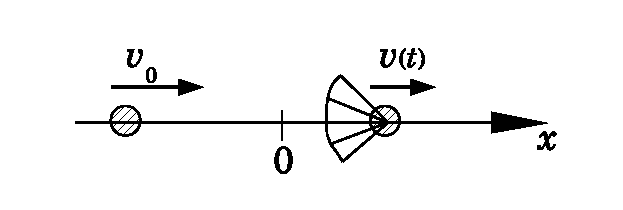
\includegraphics[width=7cm]{parachute.eps}
    \caption{等速直線運動している物体に突然空気抵抗がかかる。}\label{fig:parachute}
\end{figure}
\begin{enumerate}
\item $t<0$では, 次式が成り立つことを示せ:
\begin{eqnarray}
0=m\frac{dv}{dt}\label{eq:friction_stop1}
\end{eqnarray}
\item $0<t$では, 次式が成り立つことを示せ:
\begin{eqnarray}
-\alpha v=m\frac{dv}{dt}\label{eq:friction_stop2}
\end{eqnarray}
\item 上の式は, 関数$v(t)$に関する微分方程式だ。数学リメディアル教材を参考にして, 
この微分方程式を解け。結果は次式のようになるはずである:
\begin{eqnarray}
v(t)=v_0\exp\Bigl(-\frac{\alpha}{m}t\Bigr)\label{eq:stop_viscosity}
\end{eqnarray}
\item 関数$v(t)$のグラフを描け。
\end{enumerate}
\end{q}

このように, 空気や水などの流体\footnote{気体と液体をまとめて流体と呼ぶ。}の中で物体が速度に比例して受ける抵抗を\underline{粘性抵抗}
\index{ねんせいていこう@粘性抵抗}という。
しかしながら, 物体が大きかったり速度が速いとき, 速度の2乗に比例する
抵抗をより強く受ける。それを\underline{慣性抵抗}\index{かんせいていこう@慣性抵抗}という
\footnote{このあたりの法則は, 流体力学という物理学で説明されるが, 流体力学のほとんど
はニュートン力学を基本法則とする。}。\mv

%
\begin{q}\label{q:resistance}
粘性抵抗とは何か? 慣性抵抗とは何か?
\end{q}
\mv

%
\begin{q}\label{q:parachute2}
問\ref{q:parachute}において, パラシュートによる空気抵抗が粘性抵抗でなく慣性抵抗ならどうなるだろう? 
いま, 空気抵抗が$-\beta v^2$であるとする($\beta $は適当な定数)。
\begin{enumerate}
\item パラシュートが開いてから物体が停止するまでの間, 次式が成り立つことを示せ:
\begin{eqnarray}
-\beta\,v^2=m\frac{dv}{dt}\label{eq:parachute20}
\end{eqnarray}
\item 上の微分方程式を変数分離すると, 次式のようになることを示せ:
\begin{eqnarray}
\beta\,dt=-\frac{mdv}{v^2}\label{eq:parachute21}
\end{eqnarray}
\item これを不定積分すると, 次式のようになることを示せ($C$は積分定数):
\begin{eqnarray}
\beta\,t=\frac{m}{v}+C\label{eq:parachute22}
\end{eqnarray}
\item 以下の式が成り立つことを示せ。
\begin{eqnarray}
C=-\frac{m}{v_0}\label{eq:parachute23}
\end{eqnarray}
\item 以下の式が成り立つことを示せ。
\begin{eqnarray}
v(t)=\frac{mv_0}{v_0\,\beta\,t+m}\label{eq:parachute24}
\end{eqnarray}
\item 関数$v(t)$のグラフを描け:
\end{enumerate}
\end{q}
\mv

\begin{faq}{\small\textgt{問\ref{q:parachute}で, 
なぜ最初は力0なのですか? 力がないと進まないのでは? } ... 
物体は, \textgt{力がなくても動き続ける}のです。
等速直線運動をするのです。それが慣性の法則です。
「力がないと物体は進まない」というのは間違いです。
思い込みです。止まっている物体を動き出させる
ためには, 確かに最初に力をかけてやる必要がありますが, いったん動き出せば, 
力をかけなくても物体は勝手に動き続けるのです。}\end{faq}\mv

\begin{faq}{\small\textgt{物体が力を受けなくても等速で
動くのなら止まっている物体は力を受けて止まっているのですか?} ... 
いいえ。「止まっている」も「等速で動く」ことの一種で, 働く力は0です。}\end{faq}\mv

%
\begin{q}\label{q:raindrop}
雨粒の落下を考えよう。雨粒は重力を受けて加速しながら落下するが, 同時に空気抵抗も受けるので, 
際限なく加速することはあり得ない。また, 雨粒が十分小さければ, 空気抵抗は粘性抵抗とみなすことができる。
いま, 鉛直上向きに座標軸をとる。質量$m$の雨粒が鉛直方向に直線的に落下するとし, 時刻$t$における雨粒
の落下速度を$v(t)$とする。$v(0)=0$とする。雨粒にかかる空気抵抗(粘性抵抗)を$-\alpha v$とする
($\alpha$は適当な正の定数)。注:落下は下向きだから$v$は負であり, 空気抵抗"$-\alpha v$"は$v$にマイナスが
かかっているから正, つまり上向きである。
\begin{enumerate}
\item 雨粒に関する運動方程式は以下のようになることを示せ:
\begin{eqnarray}
-mg-\alpha v=m\frac{dv}{dt}\label{eq:raindrop1}
\end{eqnarray}
\item これを変数分離すると次式になることを示せ:
\begin{eqnarray}
\frac{dv}{g+\alpha v/m}=-dt\label{eq:raindrop2}
\end{eqnarray}
\item これを両辺を積分すると次式になることを示せ($C$は積分定数):
\begin{eqnarray}
\frac{m}{\alpha}\ln\Bigl|v+\frac{gm}{\alpha}\Bigr|=-t+C\label{eq:raindrop3}
\end{eqnarray}
\item これを$v$について解き, 特に$v(0)=0$に注意して, 次式を示せ:
\begin{eqnarray}
v(t)=\frac{mg}{\alpha}\Bigl\{\exp\Bigl(-\frac{\alpha}{m}t\Bigr)-1\Bigr\}\label{eq:raindrop4}
\end{eqnarray}
\item $v(t)$のグラフを描け。
\item 時間が十分にたって速度が一定になったときの速度を\underline{終端速度}
\index{しゅうたんそくど@終端速度}という。この場合, 終端速度は
\begin{eqnarray}v=-\frac{mg}{\alpha}\end{eqnarray}
となることを示せ。
\end {enumerate}
\end{q}
\mv

雨が降る時, 雨粒は地表面に衝撃を与える。地表を植生が覆っていれば, 
葉やリター(落ち葉等)で雨滴衝撃を吸収してくれるが, 地表に植生が無い
場合は, 雨滴衝撃で土壌侵食を起こすことがある。これは農地や, 間伐が不十分
なスギ・ヒノキ人工林などで問題になっている。\mv

粘性抵抗を受ける落下の問題は, 微粒子(穀物の粉とか, 大気汚染源の粉塵など)の運動を議論する上で
基礎的なものだ。また, 微粒子の大きさを計測する上でもこの理論がよく利用される。

\begin{comment}
では, 慣性抵抗を受ける落下運動はどうなるだろう?
\mv
\begin{figure}[h]
    \centering
    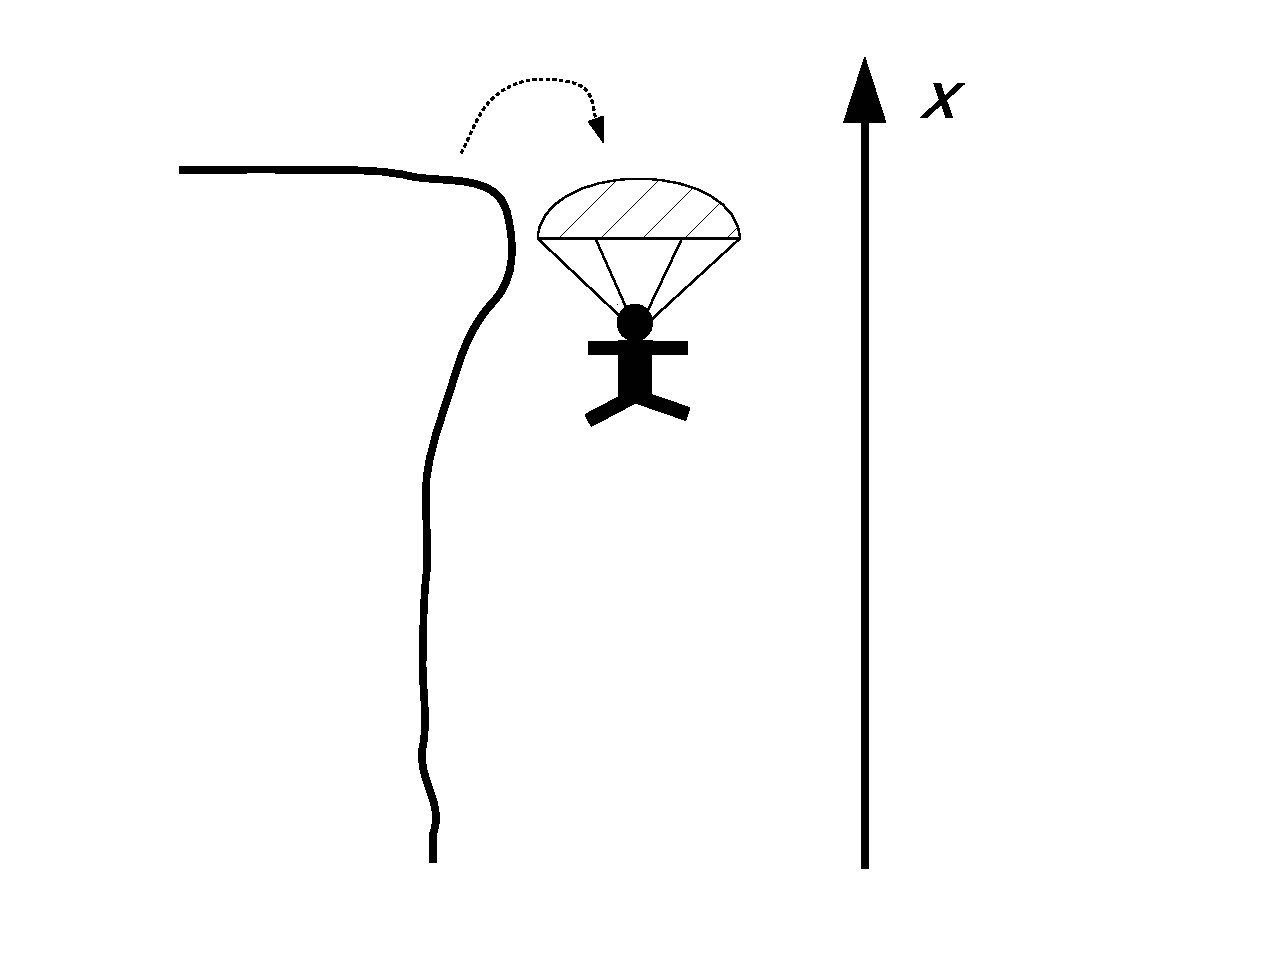
\includegraphics[width=5cm]{cliff_fall.eps}
    \caption{崖からパラシュートで降下する。詳しくは問\ref{q:parachute_energy}参照。}\label{fig:cliff_fall}
\end{figure}

\begin{q}\label{q:parachute_energy}
君は高い崖の上からパラシュートで降下しようとしている(図\ref{fig:cliff_fall})。
君は重力を受けて加速しながら落下するが, 
同時に空気抵抗も受けるので, 際限なく加速することはあり得ない。また, このような場合, 君が受ける空気抵抗は
慣性抵抗とみなすことができる。いま, 鉛直上向きに座標軸をとる。質量$m$の君が鉛直方向に直線的に落下
するとし, 時刻$t$における君の落下速度を$v(t)$とする。君にかかる空気抵抗(慣性抵抗)を$\beta v^2$とする
($\beta$は適当な正の定数)。
注:落下は下向きだが, 空気抵抗は上向き, つまり空気抵抗の符号は正である。
\begin{enumerate}
\item 君に関する運動方程式は以下のようになることを示せ:
\begin{eqnarray} 
-mg+\beta v^2=m\frac{dv}{dt}\label{eq:parachute_fall1}
\end{eqnarray} 
\item 時間が十分にたつと, 空気抵抗と重力がつりあって, 速度は一定値になるはずだ。そのとき, 
上の式で$dv/dt=0$となる。それを利用して, 終端速度の大きさ$v_{\infty}$は, 
\begin{eqnarray}v_{\infty}=\sqrt{\frac{mg}{\beta}}\end{eqnarray}
となることを示せ。(ただし, もし向きまで考えるならばこの式にマイナスが付く。ここでは向きは考えず, 大きさだけを考えている。)
\item $v_{\infty}$を使うと, 上の方程式は次式のように書き換えることができることを示せ:
\begin{eqnarray}m\frac{dv}{dt}=\beta (v^2-v_{\infty}^2)\end{eqnarray}
\item これを変数分離して部分分数展開(数学リメディアル教材参照)すると, 次式になることを示せ:
\begin{eqnarray}\Bigl(\frac{1}{v-v_{\infty}}-\frac{1}{v+v_{\infty}}\Bigr)\frac{dv}{2v_{\infty}}=\frac{\beta}{m}dt\end{eqnarray}
\item 両辺積分すると次式になることを示せ(ここで$C$は積分定数)
\begin{eqnarray}\frac{1}{2v_{\infty}}\ln\Bigl|\frac{v-v_{\infty}}{v+v_{\infty}}\Bigr|=\frac{\beta}{m}t+C\label{eq:parachute_fall5}
\end{eqnarray}
\item 初速度$v(0)$を0とすると, 次式のようになることを示し, $v(t)$のグラフを描け。
\begin{eqnarray}v=-v_{\infty}\tanh\Bigl(v_{\infty}\frac{\beta}{m}t\Bigr)\end{eqnarray}
ただし, $\tanh x$は「双曲線関数」と呼ばれる関数の一種であり, その定義は, 
\begin{eqnarray}\tanh x=\frac{e^x-e^{-x}}{e^x+e^{-x}}\end{eqnarray}
である。$\tanh$を「ハイパボリック・タンジェント」と呼ぶ。
\end{enumerate}
\end{q}
\mv
\end{comment}

\section{運動の三法則と哲学}

本章の最後に, ちょっと哲学っぽいことを考えよう。運動の三法則は, 
物体の運動を正確に予測することができる, ということを世界に示した。
それは, 未来を占うのにオカルト的な力が必要だと信じていた人に, 
ちょっとしたショックを与えただろう。そこで生まれたのが
「ラプラスの悪魔」という概念である。\mv

\begin{q}\label{q:Laplace_demon}
「ラプラスの悪魔」とは何か? それは近代の宗教や思想にどのような影響を与えただろうか? 
それは物理学的にはどのように反駁(はんばく)されたか? 
\end{q}
\hv
\begin{comment}
\begin{q}\label{q:cheat_experiment}
ある高校には, 地元の有名な学習塾に通う生徒が大勢いた。彼らは学校の理科の
実験で, 配られた記録用紙に塾で習った実験結果を手早く書き, 余った時間を
テスト対策の内職勉強をしていた。彼らは, 結果がわかりきった実験をわざわざ
繰り返す必要は無いし, 時間の無駄であるという。彼らの行為や考え方について
自由に論じよ。\end{q}
\hv
\end{comment}

\begin{exq} 質量$m$の質点に, $x$軸の正の方向に$F=Ae^{-kt}$という力がかかっている。
ここで, $A, k$は正の定数であり, $t$は時刻。質点の速度$v$を$t$の関数として
表せ。ただし初速度を0とする。\end{exq}

\begin{exq} 2つの質点A, Bが, 質量を持たないバネでつながれている。質点Aを水平方向にひっぱる
ことで, これらを摩擦の無い水平面上で, 加速度0.50~m~s$^{-2}$で等加速度直線運動をさせる。質点A, Bの
質量はそれぞれ2.0~kgと3.0~kgとし, バネ定数は4.5~N/mとする。バネの伸びを求めよ。
ヒント: 2つの質点のそれぞれについて運動方程式を立てる。\end{exq}

\begin{exq} ジャンボジェット機(ボーイングB747)が, 成田空港の, 
幅60~mの滑走路に, その中心線を目指ざして着陸しようとしている。あと5秒で
車輪が滑走路につくというとき, 突然, 横から$v=10$~m/sの突風が吹いてきた。この飛行機は
無事に滑走路内に着陸できるか? 根拠と共に示せ。ただし, 物体が風から受ける力
(慣性抵抗)の大きさ$F$は, $F=\rho v^2 S C_{\text{D}}/2$と表せることが知られている。
ここで$\rho$は空気の密度であり, $S$は風の方向に投影した物体の面積である。$C_{\text{D}}$は「抗力係数」
と呼ばれる無次元の数で, 物体の形状や風の性質に依存するが, おおよそ0.5から2程度の値
である。また, ジャンボジェットの質量は乗客も含めて約300~t, ジャンボ・ジェットの
胴体は全長70~m, 直径8~m程度である。\end{exq}




\section{解答}

\noindent{\textbf{答}}\ref{q:motion1condition}
(1) AはCの十分条件。必要条件ではない。静止していれば合力はゼロだが, 
合力がゼロであっても静止していない場合(${\bf 0}$以外の速度での等速直線運動)があり得る。
(2) BはCの必要十分条件。
(3) BはAの必要条件。十分条件ではない。静止は等速直線運動の一種(速度${\bf 0}$での等速直線運動)。
\mv

%\noindent{\textbf{答}}\ref{q:escalator} 略。ヒント: 
%エスカレーターが突然停止したらどうなるか?\mv

% 運動の三法則とは何か? 
%\noindent{\textbf{答}}\ref{q:Newton_3laws} 略。
%\vspace{0.2cm}

\noindent{\textbf{答}}\ref{q:NewtonLaw_mistake} 
(1) 間違い。「AはBから, 同じ\textgt{大きさで逆向きの}力を受ける」
(2) 正しい。質点が等速直線運動をしているとき, 加速度${\bf a}$は${\bf 0}$である。
従って, 第二法則より, 物体にかかる合力${\bf F}$は${\bf 0}$である。
(3) 直線方向の運動(1次元の運動)に限定すれば正しい。しかし一般には, 
力も加速度もベクトルなので, $F$と$a$のかわりに${\bf F}$と${\bf a}$と
書かねばならない。
\mv

% 運動量とは何か? 
%\noindent{\textbf{答}}\ref{q:def_momentum} 質量($m$)と速度(${\bf v}$)の積$m{\bf v}$。
%\vspace{0.2cm}

% 地表付近で重力だけを受けて上下運動をする, 
\noindent{\textbf{答}}\ref{q:freefall0}
\begin{enumerate}
\item \eref{eq:gravity_earth}より, 質点には鉛直下向きに大きさ$mg$の重力がかかる。
座標系は鉛直上向きを正にとっているので, この重力$F$は$F=-mg$
と書ける\footnote{\eref{eq:gravity_earth}は力の向きは考えず力の大きさだけを
考えていたことに注意せよ。}。重力以外の力は働いていない。従って運動方程式より, 
$-mg=ma$
\item \eref{eq:constacc_vx}, \eref{eq:constacc_x}で, $a_x$を$-g$, $v_x$を$v$とすれば, 与式を得る。
\item $x_0=0$, $v_0=0$とすればよい。
\end{enumerate}
\mv


% 地表付近で, 初速度0で質点を投下し, 自由落
\noindent{\textbf{答}}\ref{q:freefall1} 初期位置を原点とし, 鉛直上向きに$x$軸をとる。時刻$t$における位置と速度をそれぞれ$x(t)$, $v(t)$とする。
(1) \eref{eq:freefallveq0}, \eref{eq:freefallxeq0}で$t=10$ sとすれば, $v=-98$~m~s$^{-1}$, $x=-490$~m。従って落下距離は490~m。
(2) 加速度が$-g$の等加速度直線運動なので$v(t)=-gt$。従って$t=-v(t)/g$。
いま, $v(t)=-340$~m~s$^{-1}$なので, $t=340$~m~s$^{-1}$/(9.8~m~s$^{-2}$) =35~s。従って約35秒後。
\eref{eq:freefallxeq0}で$t=35$ sとすれば, $x=-6000$~m。従って, 約6000~m落下する。
\vspace{0.2cm}

% プロ野球投手が初速度$v_0=40$m/s(約140km/hに相当)でボ
\noindent{\textbf{答}}\ref{q:baseball0}\\
\eref{eq:freefallxeq}で, $x_0=0$とすれば, 
\begin{eqnarray}
x(t)&=&v_0t-\frac{1}{2}gt^2=-\frac{1}{2}g\Bigl(t^2-\frac{2v_0}{g}t\Bigr)\\
    &=&-\frac{1}{2}g\Bigl(t-\frac{v_0}{g}\Bigr)^2+\frac{v_0^2}{2g}
\end{eqnarray}
従って, $t=v_0/g$のとき, 最高高度$v_0^2/(2g)$に到達する。ここで$v_0=40$~m~s$^{-1}$とすると, 最高高度は, 
\begin{eqnarray}
\frac{(40\text{ m s}^{-1})^2}{2\times9.8\text{ m s}^{-2}} =82\text{ m}
\end{eqnarray}
すなわち, 約80~mの高さまで届く。
(グラフは省略。)
\vspace{0.2cm}

% カーリングというスポーツでは, 氷の上で石(ストーン)を滑らせて当てあう
\noindent{\textbf{答}}\ref{q:curling}
\begin{enumerate}
\item 手放された後のストーンに働く力は, 氷面からうける
動摩擦力$F_{\text m}$と, 重力である。重力は氷面から受ける垂直抗力と打ち消し合う。また, 摩擦力$F_{\text m}$は
$x$軸の逆方向に働く。従って, ストーンに働く力の総和$F$は, $F=-F_{\text m}$となる。加速度を$a$とすると, 
運動方程式は, 
\begin{eqnarray}
-F_{\text m}=ma
\end{eqnarray}
\item 前小問より, $a=-F_{\text m}/m$となるが, これは時刻によらない一定値。
すなわちこれは等加速度直線運動である。
\eref{eq:constacc_vx}, \eref{eq:constacc_x}で, $a_x$を$-F_{\text m}/m$, 
速度$v_x$を$v$とすれば, 
\begin{eqnarray}
v&=&v_0-\frac{F_{\text m}}{m}\,t\label{eq:stonev}\\
x&=&v_0t-\frac{F_{\text m}}{2m}\,t^2\label{eq:stonex}
\end{eqnarray}
となる。ここで$x(0)=0$, $v(0)=v_0$を用いた。グラフは図\ref{fig:stone}のようになる。
\begin{figure}[h]
    \centering
    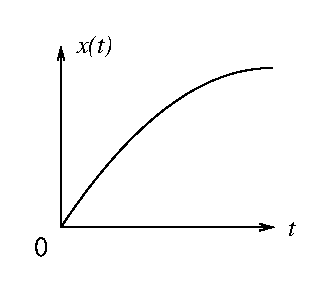
\includegraphics[width=4cm]{stone.eps}
    \caption{カーリングのストーンの運動。}\label{fig:stone}
\end{figure}
\item ストーンが停止した時刻を$t$, そのときの位置を$x$とすると, 
そのとき速度$dx/dt$は0になるから, 
式(\ref{eq:stonev})より, 
\begin{eqnarray}
0=-\frac{F_{\text m}}{m}\,t+v_0
\end{eqnarray}
従って, $t=mv_0/F_{\text m}$。これを式(\ref{eq:stonex})に代入すると, 
\begin{eqnarray}
x=\frac{mv_0^2}{2F_{\text m}}\label{eq:stonexx}
\end{eqnarray}
従って, 
\begin{eqnarray}
F_{\text m}=\frac{mv_0^2}{2x}\label{eq:stoneFm}
\end{eqnarray}
ここで, $x=20$~m, $m=20$~kg, $v_0=1.5$~m~s$^{-1}$とすれば, $F_{\text m}=1.1$ N。
\item クーロンの摩擦法則(式(\ref{eq:friction_m}))より, 動摩擦係数$\mu'$について, 
\begin{eqnarray}
F_{\text m}=\mu' N\label{eq:curling_Fm}
\end{eqnarray}
が成り立つ。ここで$N$はストーンと氷の接触面に垂直に働く力であり, 今の場合は$N=mg$である。従って, 
$F_{\text m}=\mu' mg$である。従って, 上の結果から, 
$\mu'=F_{\text m}/(mg)=5.7\times10^{-3}$。(無次元
なので単位は不要)
\item 式(\ref{eq:stonexx})より, 停止するまでの距離$x$は, 初速度$v_0$の2乗に比例する。
$x$を20~mから25~mにするとき, $x$は1.25倍になるが, そのためには$v_0$が$\sqrt{1.25}=1.12$倍
になればよい。従って, $v_0$は$\sqrt{1.25}\times1.5$~m~s$^{-1}$=1.68~m~s$^{-1}$。つまり, 約1.7~m~s$^{-1}$にすればよい。
\item \eref{eq:stonexx}と\eref{eq:curling_Fm}で$F_{\text m}$を消去し, $F_{\text m}=\mu' mg$を使えば, 
\begin{eqnarray}
x=\frac{v_0^2}{2\mu'g}\label{eq:stonexx2}
\end{eqnarray}
となる。従って$x$は質量に依存しない。従って, 30~kgだろうが何kgだろうが, 
摩擦の条件(氷の表面状態とストーンの底面材質)が同じなら, 前小問で
求めた初速度(約1.7~m~s$^{-1}$)でよい。
\end{enumerate}
\vspace{0.2cm}

\begin{faq}{\small\textgt{問\ref{q:curling}(6)に驚きました。
重い物体が, 軽い物体と同じ初速度で同じ距離で止まるのですか?}
... そうです。不思議ですね。これは, 力が摩擦力だからです。この場合の
摩擦力は, 重力に比例します。重い物体にはそのぶん, 垂直効力が
大きくなるため, 大きな摩擦力がかかるのです。つまり$F=ma$の左辺の$F$が$m$に比例するため, 
右辺の$ma$の$m$と打ち消し合って, 結果的に質量の影響は
無くなるのです。}\end{faq}\mv


\noindent{\textbf{答}}\ref{q:increase_force} 
質量を$m$, 時刻を$t$, 力を$F(t)$とする。力は時刻に比例するので, 
\begin{eqnarray}
F(t)=bt\label{eq:increase_force}
\end{eqnarray}
と書ける($b$は適当な定数)。運動方向に$x$軸をとり, 
位置を$x(t)$, 速度を$v(t)$, 加速度を$a(t)$とする。運動方程式より, $F(t)=ma(t)$。
これに\eref{eq:increase_force}を代入して変形すると,
\begin{eqnarray}
a(t)=\frac{bt}{m}\label{eq:increase_force2}
\end{eqnarray}
となる。\eref{eq:vxfromax}のように考えて($a_x$, $v_x$はここでは$a$, $v$), 
\begin{eqnarray}
v(t)&=&v(0)+\int_{0}^{t}a(t)\, dt\label{eq:increase_force3}
\end{eqnarray}
である。ここで$v(0)=0$と, \eref{eq:increase_force2}を代入して, 
\begin{eqnarray}
v(t)&=&\int_{0}^{t}\frac{bt}{m}\, dt=\frac{bt^2}{2m}\label{eq:increase_force4}
\end{eqnarray}
また, \eref{eq:xfromvx}のように考えて, 
\begin{eqnarray}
x(t)&=&x(0)+\int_{0}^{t}v(t)\, dt
\end{eqnarray}
である。ここで$x(0)=0$と, \eref{eq:increase_force4}を代入して, 
\begin{eqnarray}
x(t)&=&\int_{0}^{t}\frac{bt^2}{2m}\, dt=\frac{bt^3}{6m}\label{eq:increase_force6}
\end{eqnarray}
さて, \eref{eq:increase_force}で$t=3.0$~sのときを考えると, 
6.0~N$=b\times$2.0~sだから, $b=3.0$~N/s。これと, $m$=2.0~kg, $t=$4.0~sを
\eref{eq:increase_force6}に代入すると, 
\begin{eqnarray}
x(4.0\text{ s})&=&\frac{(3.0\text{ N/s})(4.0\text{ s})^3}{6\times 2.0\text{ kg}}=16\text{ m}
\end{eqnarray}
\mv

% 質量$m$の物体が, 速度$v_0$で等速直線運動している
\noindent{\textbf{答}}\ref{q:parachute}
\begin{enumerate}
\item $t<0$では等速直線運動をしているから, 慣性の法則より, 働く力(の総和)は0である。
従って, 運動方程式より, 式(\ref{eq:friction_stop1})が成り立つ。
\item $0<t$ではパラシュートによる空気抵抗力$F=-\alpha v$がかかる。従って, 運動方程式より, 式(\ref{eq:friction_stop2})が成り立つ。
\item 式(\ref{eq:friction_stop2})を変数分離すると, 
\begin{eqnarray}-\alpha dt=m\frac{dv}{v}\end{eqnarray}
さて, 上の式を両辺, 積分すると($C$は積分定数), 
\begin{eqnarray}-\alpha t=m\ln|v|+C\end{eqnarray}
($C'$は$C$とは別の定数)。従って, 
\begin{eqnarray}v=\pm \exp\Bigl(-\frac{\alpha}{m}t+C'\Bigr)=\pm C'\,\exp\Bigl(-\frac{\alpha}{m}t\Bigr)\,\,\,\end{eqnarray}
ここで$t=0$のとき$v=v_0$だから, 
\begin{eqnarray}\pm \exp C'=v_0\end{eqnarray}
従って, 
\begin{eqnarray}v=v_0 \exp\Bigl(-\frac{\alpha}{m}t\Bigr)\end{eqnarray}
\item 図\ref{fig:viscos}のようになる。
\begin{figure}[h]
    \centering
    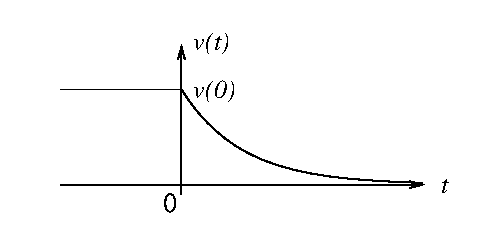
\includegraphics[width=7cm]{viscos.eps}
    \caption{粘性抵抗を受けて減速する物体の運動。}\label{fig:viscos}
\end{figure}
\end{enumerate}
\vspace{0.2cm}

% 粘性抵抗とは何か? 慣性抵抗とは何か?
%\noindent{\textbf{答}}\ref{q:resistance}\\
%粘性抵抗とは, 流体の中で, 物体が速度に比例して受ける抵抗力。慣性抵抗とは, 物体が流体の中で速度の二乗
%に比例して受ける抵抗力。
%\vspace{0.2cm}

% 前問において, パラシュートによる空気抵抗が粘性抵抗でなく慣性抵抗な
\noindent{\textbf{答}}\ref{q:parachute2}
(1) $0<t$ではパラシュートによる空気抵抗力$F=-\beta v^2$がかかる。従って, 運動方程式より, \eref{eq:parachute20}が成り立つ。
(2), (3) 略。
(4) \eref{eq:parachute22}で, $t=0$とすれば, $0=m/v(0)+C$。従って$C=-m/v(0)$。
(5) \eref{eq:parachute23}を\eref{eq:parachute22}に入れて$v$についてとけば, 
\eref{eq:parachute24}が成り立つ。(各自, 計算してみよ) 
(6) 図\ref{fig:inert_v}のようになる。
\begin{figure}[h]
    \centering
    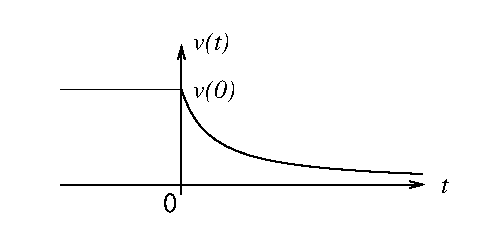
\includegraphics[width=7cm]{inert_v.eps}
    \caption{慣性抵抗を受けて減速する物体の運動。}\label{fig:inert_v}
\end{figure}
\vspace{0.2cm}


% 雨粒の落下を考えよう。雨粒は重力を受け
\noindent{\textbf{答}}\ref{q:raindrop}
\begin{enumerate}
\item 雨粒にかかる力は, 重力($-mg$)と粘性抵抗($-\alpha v$)の和。
従って, 運動方程式より, \eref{eq:raindrop1}が成り立つ。
\item \eref{eq:raindrop1}の両辺を$m$で割ると, 
\begin{eqnarray}-g-\frac{\alpha v}{m}=\frac{dv}{dt}\end{eqnarray}
両辺に$dt$をかけ, さらに両辺を$g+\alpha v/m$で割ると, 
\begin{eqnarray}-dt=\frac{dv}{g+\alpha v/m}\end{eqnarray}
この左辺と右辺を入れ替えると, \eref{eq:raindrop2}を得る。
\item \eref{eq:raindrop2}の両辺に積分記号$\int$をつける:
\begin{eqnarray}\int\frac{dv}{g+\alpha v/m}=-\int dt\end{eqnarray}
この左辺の不定積分は, 
\begin{eqnarray*}
\int\frac{dv}{(\alpha/m)(v+gm/\alpha)}=\frac{m}{\alpha}\int\frac{dv}{v+gm/\alpha}\\
=\frac{m}{\alpha}\ln\Bigr|v+\frac{gm}{\alpha}\Bigl|+C_1
\end{eqnarray*}
となる($C_1$は積分定数)。右辺の不定積分は, $-t+C_2$となる($C_2$は積分定数)。これらをまとめて, 
\begin{eqnarray}
\frac{m}{\alpha}\ln\Bigl|v+\frac{gm}{\alpha}\Bigr|+C_1=-t+C_2
\end{eqnarray}
となる。$C_1$を右辺に移項し, $C_2-C_1=C$とおけば, \eref{eq:raindrop3}を得る。
\item \eref{eq:raindrop3}より, 
\begin{eqnarray}
\ln\Bigr|v+\frac{gm}{\alpha}\Bigl|=-\frac{\alpha}{m}(t-C)
\end{eqnarray}
従って, 
\begin{eqnarray}
v+\frac{gm}{\alpha}=\pm\exp\Bigl[-\frac{\alpha}{m}(t-C)\Bigr]
\end{eqnarray}
従って, 
\begin{eqnarray}
v=\pm\exp\Bigl[-\frac{\alpha}{m}(t-C)\Bigr]-\frac{gm}{\alpha}\label{eq:randrop_ans11}
\end{eqnarray}
ここで$t=0$, $v=0$とおけば, 
\begin{eqnarray}
0=\pm\exp\Bigl[\frac{\alpha}{m}C\Bigr]-\frac{gm}{\alpha}
\end{eqnarray}
従って, 
\begin{eqnarray}
\pm\exp\Bigl[\frac{\alpha}{m}C\Bigr]=\frac{gm}{\alpha}
\end{eqnarray}
となる(左辺の$\pm$も含めて右辺のように決まる)。これを\eref{eq:randrop_ans11}に代入して, 
\begin{eqnarray}
v=\frac{gm}{\alpha}\exp\Bigl[-\frac{\alpha}{m}\,t\Bigr]-\frac{gm}{\alpha}
\end{eqnarray}
これを整理すると\eref{eq:raindrop4}を得る。
\item 図\ref{fig:viscos_fall}のようになる。
\begin{figure}[h]
    \centering
    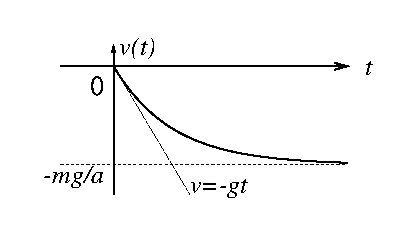
\includegraphics[width=7cm]{viscos_fall.eps}
    \caption{粘性抵抗を受ける落下。}\label{fig:viscos_fall}
\end{figure}
\item \eref{eq:raindrop4}において$t$の$\infty$への極限で, $v$は$-mg/\alpha$に近づく。
あるいは, 終端速度では速度は時間とともに変わらないから, \eref{eq:raindrop1}の右辺を
0とおけば, 同じく$v=-mg/\alpha$を得る。
\end{enumerate}
\vspace{0.2cm}

\begin{comment}
% 君は高い崖の上からパラシュートで降下しようとしている
\noindent{\textbf{答}}\ref{q:parachute_energy}
\begin{enumerate}
\item 君にかかる力は, 重力($-mg$)と空気抵抗力($\beta v^2$)の合力である。
そこで, 
\begin{eqnarray}F=-mg+\beta v^2\end{eqnarray}
として, 1次元の運動方程式$F=mdv/dt$に代入すれば, 与式を得る。
\item $v$の大きさが一定値$v_\infty$に至ったとして, $dv/dt=0$とすれば, 式(\ref{eq:parachute_fall1})より, $-mg+\beta v^2=0$。
従って, このとき, $|v|=\sqrt{mg/\beta}=v_\infty$。
\item 略($v_\infty$を使って式(\ref{eq:parachute_fall1})から$g$を消せばよい)。
\item 略。
\item 略。
\item \eref{eq:parachute_fall5}より, 
\begin{eqnarray}
\frac{v-v_\infty}{v+v_\infty}=\pm\exp\Bigl(2v_\infty\bigl(\frac{\beta}{m}\,t+C\bigr)\Bigr)
\end{eqnarray}
これに, $t=0$, $v=0$を代入して左辺=右辺となるようにするには, 右辺の符号はマイナスであり, かつ, $C=0$とするしかない。従って, 
\begin{eqnarray}
\frac{v-v_\infty}{v+v_\infty}=-\exp\Bigl(2v_\infty\frac{\beta}{m}\,t\Bigr)
\end{eqnarray}
これを$v$について解けば(詳細略), 次式のようになる:
\begin{eqnarray}
v=-v_\infty\frac{\exp\Bigl(2v_\infty\frac{\beta}{m}\,t\Bigr)-1}{\exp\Bigl(2v_\infty\frac{\beta}{m}t\Bigr)+1}
\end{eqnarray}
右辺の分子と分母にそれぞれ
\begin{eqnarray}
\exp\Bigl(-v_\infty\frac{\beta}{m}\,t\Bigr)
\end{eqnarray}
をかければ, 
\begin{eqnarray*}
v=-v_\infty\frac{\exp\Bigl(v_\infty\frac{\beta}{m}\,t\Bigr)-\exp\Bigl(-v_\infty\frac{\beta}{m}\,t\Bigr)}{\exp\Bigl(v_\infty\frac{\beta}{m}\,t\Bigr)+\exp\Bigl(-v_\infty\frac{\beta}{m}\,t\Bigr)}
\end{eqnarray*}
となる。この右辺は, 
\begin{eqnarray}
-v_\infty\tanh\Bigl(v_\infty\frac{\beta}{m}\,t\Bigr)
\end{eqnarray}
である。グラフは図\ref{fig:inert_fall}のとおり:
\begin{figure}[h]
    \centering
    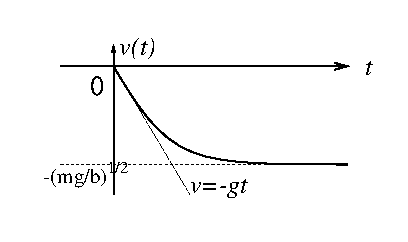
\includegraphics[width=7cm]{inert_fall.eps}
    \caption{慣性抵抗を受ける落下。}\label{fig:inert_fall}
\end{figure}
\end{enumerate}
\end{comment}

%
\noindent{\textbf{答}}\ref{q:Laplace_demon}\\
略(各自, 調べよ)。
\hv


\begin{faq}{\small\textgt{摩擦のない面に10~tくらいの
物体がのって静止しているとします。摩擦がなければ, この物体を
面と平行な方向に動かし始めるには, ほんの少し力をかけて
やるだけで良いのでしょうか。イメージできない。} ... 
はいそうです。実際, 小惑星探査機「はやぶさ」は
500~kgほどですが, それを動かすイオンエンジンは1円玉
を持ち上げるくらいの力しかなかったらしいですよ。}\end{faq}

\begin{comment}
\begin{faq}{\small\textgt{ラプラスの悪魔にびっくりしました。} ... 
私も若い頃, ラプラスの悪魔を知って, 自分の人生は
もう決まってるのかと, 一瞬, 凹みました。}\end{faq}

\begin{faq}{\small\textgt{解答をみるとわかるんですけど, 
一から自分で解答を作り出せません。} ... 基本から丁寧に
理解することが重要で, 必ずしも「一から作り出す」ことには
こだわらなくていいです。受験勉強じゃないんだし, 
新しいことを学んでいるのだから。}\end{faq}\mv
\end{comment}

